%%%%%%%%%%%%%%%%%%%%%%%%%%%%%%% beamer %%%%%%%%%%%%%%%%%%%%%%%%%%%%%%%%%%%%%%%%%%%%%%%%%
% To run - pdflatex filename.tex
%      acroread filename.pdf
%%%%%%%%%%%%%%%%%%%%%%%%%%%%%%%%%%%%%%%%%%%%%%%%%%%%%%%%%%%%%%%%%%%%%%%%%%%%%%%%%%%%%%%%

\documentclass[compress,oilve]{beamer}
\mode<presentation>

\usetheme[]{CambridgeUS}
% other themes: AnnArbor, Antibes, Bergen, Berkeley, Berlin, Boadilla, boxes, CambridgeUS, Copenhagen, Darmstadt, default, Dresden, Frankfurt, Goettingen,
% Hannover, Ilmenau, JuanLesPins, Luebeck, Madrid, Maloe, Marburg, Montpellier, PaloAlto, Pittsburg, Rochester, Singapore, Szeged, classic

\usecolortheme{beaver}
% color themes: albatross, beaver, beetle, crane, default, dolphin,  fly, lily, orchid, rose, seagull, seahorse, sidebartab, whale, wolverine

\usefonttheme{professionalfonts}
% font themes: default, professionalfonts, serif, structurebold, structureitalicserif, structuresmallcapsserif


\hypersetup{pdfpagemode=FullScreen} % makes your presentation go automatically to full screen

% define your own colors:
\definecolor{Red}{rgb}{1,0,0}
\definecolor{Blue}{rgb}{0,0,1}
\definecolor{Green}{rgb}{0,1,0}
\definecolor{magenta}{rgb}{1,0,.6}
\definecolor{lightblue}{rgb}{0,.5,1}
\definecolor{lightpurple}{rgb}{0.8, 0.6, 0.9}
\definecolor{gold}{rgb}{.6,.5,0}
\definecolor{orange}{rgb}{1,0.4,0}
\definecolor{hotpink}{rgb}{1,0,0.5}
\definecolor{newcolor2}{rgb}{.5,.3,.5}
\definecolor{newcolor}{rgb}{0,.3,1}
\definecolor{newcolor3}{rgb}{1,0,.35}
\definecolor{darkgreen1}{rgb}{0, .35, 0}
\definecolor{darkgreen}{rgb}{0, .6, 0}
\definecolor{darkred}{rgb}{.75,0,0}
\definecolor{skyblue}{HTML}{75bbfd}

\definecolor{olive}{cmyk}{0.64,0,0.95,0.4}
\definecolor{purpleish}{cmyk}{0.75,0.75,0,0}

% can also choose different themes for the "inside" and "outside"

% \usepackage{beamerinnertheme_______}
% inner themes include circles, default, inmargin, rectangles, rounded

% \usepackage{beamerouterthemesmoothbars}
% outer themes include default, infolines, miniframes, shadow, sidebar, smoothbars, smoothtree, split, tree


\useoutertheme[subsection=true, height=40pt]{smoothbars}

% to have the same footer on all slides
%\setbeamertemplate{footline}[text line]{STUFF HERE!}
\setbeamertemplate{footline}[text line]{} % makes the footer EMPTY
% include packages
%

%show the page numbers in footnote
%\addtobeamertemplate{navigation symbols}{}{%
%	\usebeamerfont{footline}%
%	\usebeamercolor[fg]{footline}%
%	\hspace{1em}%
%	\insertframenumber/\inserttotalframenumber
%}

\setbeamercolor{footline}{fg=purpleish}
\setbeamerfont{footline}{series=\bfseries}

%add color to curent subsection
\setbeamertemplate{section in head/foot}{\hfill\tikz\node[rectangle, fill=darkred, rounded corners=1pt,inner sep=1pt,] {\textcolor{white}{\insertsectionhead}};}
\setbeamertemplate{section in head/foot shaded}{\textcolor{darkred}{\hfill\insertsectionhead}}

% Remove bullet of subsections
\setbeamertemplate{headline}
{%
	\begin{beamercolorbox}{section in head/foot}
		\insertsectionnavigationhorizontal{\textwidth}{}{}
	\end{beamercolorbox}%
}


% modify headlline, specially headline size
\setbeamertemplate{headline}{%
	\leavevmode%
	\hbox{%
		\begin{beamercolorbox}[wd=\paperwidth,ht=3.5ex,dp=1.125ex]{palette quaternary}%
			\insertsectionnavigationhorizontal{\paperwidth}{}{\hskip0pt plus1filll}
		\end{beamercolorbox}%
	}
}

\setbeamertemplate{footline}{%
	\leavevmode%
	\hbox{\begin{beamercolorbox}[wd=.5\paperwidth,ht=2.5ex,dp=1.125ex,leftskip=.3cm plus1fill,rightskip=.3cm]{author in head/foot}%
			\usebeamerfont{author in head/foot}\insertshortauthor ~ \insertshortinstitute
		\end{beamercolorbox}%
		\begin{beamercolorbox}[wd=.5\paperwidth,ht=2.5ex,dp=1.125ex,leftskip=.3cm,rightskip=.3cm plus1fil]{title in head/foot}%
			\usebeamerfont{title in head/foot}\insertshorttitle\hfill\insertframenumber\,/\,\inserttotalframenumber
	\end{beamercolorbox}}%
	\vskip0pt%
}


%\setbeamertemplate{navigation symbols}{}

\title{Linear Regression}
\author{ML Instruction Team, Fall 2022}
\institute[]{CE Department \newline  Sharif University of Technology \newline \newline}
\date[\today]{}
%\titlegraphic{\includegraphics[scale=.35]{example-image}}



%Write \usepackage{etex} just after the \documentclass line (it should be the first loaded package).
\usepackage{etex}
\usepackage{subcaption}
\usepackage{multicol}
\usepackage{amsmath}
\usepackage{epsfig}
\usepackage{graphicx}
\usepackage[all,knot]{xy}
\xyoption{arc}
\usepackage{url}
\usepackage{multimedia}
\usepackage{hyperref}
\hypersetup{colorlinks,linkcolor=blue,citecolor=redorange,urlcolor=darkred}
\usepackage{multirow}
\usepackage[font={scriptsize}]{caption}
\usepackage{pgf}
\usepackage{fontspec}
%\setsansfont[Scale=MatchLowercase, BoldFont = * Bold, ItalicFont = * Italic]{Caladea}

%\usepackage{enumitem,xcolor}
%\newcommand{\labelitemi}{$\blacksquare$}
%\newcommand{\labelitemii}{$\diamond$}
%\newcommand{\labelitemiii}{$\square$}
%\newcommand{\labelitemiv}{$\ast$}
%\setbeamercolor*{item}{fg=red}


\usefonttheme{professionalfonts} 
\setbeamertemplate{itemize item}{\color{skyblue}$\blacksquare$}
\setbeamertemplate{itemize subitem}{\color{hotpink}$\blacktriangleright$}
\setbeamertemplate{itemize subsubitem}{\color{orange}$\bullet$}


\usepackage{anyfontsize}
\usepackage{t1enc}
\usepackage{tikz}
\usetikzlibrary{calc,trees,positioning,arrows,chains,shapes.geometric,decorations.pathreplacing,decorations.pathmorphing,shapes,matrix,shapes.symbols}



\newtheorem{proposition}[theorem]{Proposition}
\newtheorem{remark}[theorem]{Remark}
\newtheorem{assumption}[theorem]{Assumption}

\usepackage{xcolor}
\newcommand{\tc}[2]{
	\textcolor{#1}{\hspace{-2pt}#2\hspace{-2pt}}
}

%\usepackage{fontspec, unicode-math}
%\setmainfont[Scale=0.9]{Nimbus Roman No9 L}
%\setmonofont[Scale=0.9]{Monaco}
\setsansfont[Scale=1]{Times New Roman}

\newcommand{\vect}[1]{\boldsymbol{#1}}

\definecolor{strings}{rgb}{.624,.251,.259}
\definecolor{keywords}{rgb}{.224,.451,.686}
\definecolor{comment}{rgb}{.322,.451,.322}


%\usepackage{smartdiagram}
%\usesmartdiagramlibrary{additions}
%%%%%%%%%%%%%%%%%%%%%%%%%%%%%%%%%%%%%%%%%%%%%%%%%%%%%%%%%%%%%%%%%%%%%%%%%%%%%%%%%%%%%%%%%%%%
%%%%%%%%%%%%%%%%%%%%%%%%%%%%%% Title Page Info %%%%%%%%%%%%%%%%%%%%%%%%%%%%%%%%%%%%%%%%%%%
%%%%%%%%%%%%%%%%%%%%%%%%%%%%%%%%%%%%%%%%%%%%%%%%%%%%%%%%%%%%%%%%%%%%%%%%%%%%%%%%%%%%%%%%%%


%%%%%%%%%%%%%%%%%%%%%%%%%%%%%%%%%%%%%%%%%%%%%%%%%%%%%%%%%%%%%%%%%%%%%%%%%%%%%%%%%%%%%%%%%%
%%%%%%%%%%%%%%%%%%%%%%%%%%%%%% Begin Your Document %%%%%%%%%%%%%%%%%%%%%%%%%%%%%%%%%%%%%%%
%%%%%%%%%%%%%%%%%%%%%%%%%%%%%%%%%%%%%%%%%%%%%%%%%%%%%%%%%%%%%%%%%%%%%%%%%%%%%%%%%%%%%%%%%%
\begin{document}
	
%%%%%%%%%%%%%%%%%%%%%%%%%%%%%%%%%%%%%%%%%%%%%%%%%%%%%%%%%%%%%%%%%%%%%%%%%%%%%%%%%%%%%%%%%%
\fontsize{9}{9}
\begin{frame}[noframenumbering, plain]
	\titlepage
\end{frame}

%%%%%%%%%%%%%%%%%%%%%%%%%%%%%%%%%%%%%%%%%%%%%%%%%%%%%%%%%%%%%%%%%%%%%%%%%%%%%%%%%%%%%%%%%%
\section{Introduction}
%%%%%%%%%%%%%%%%%%%%%%%%%%%%%%%%%%%%%%%%%%%%%%%%%%%%%%%%%%%%%%%%%%%%%%%%%%%
\frame{\frametitle{Formulation}
	\begin{itemize}
		
		\item We generally formulate the linear regression model in matrix form:
		
				\begin{equation*}
			Y=X \beta+\epsilon
		\end{equation*}
	
		where the target value $y_i$ can be evaluated by	
		\begin{equation*}
			y_i=\beta_0+\beta_1 x_{i 1}+\ldots+\beta_n x_{i n}+\epsilon_i
		\end{equation*}
	
			\item $Y$ represents a vector of length $n$ containing the observed values $Y=\left(y_1, \ldots, y_m\right)^T$.
	
		\item $\beta$ is a vector for the parameters $\beta=\left(\beta_0, \ldots, \beta_n\right)^T$.
		
		\medskip
		\item $\epsilon$ is a vector for the errors
		$\epsilon=\left(\epsilon_1, \ldots, \epsilon_m\right)^T$.
		
		\medskip
		\item $X$ is a matrix of the features in which the column of ones incorporates the intercept.
		
		\begin{equation*}
			X=\left(\begin{array}{ccccc}
				1 & x_{11} & x_{12} & \ldots & x_{1 n} \\
				1 & x_{21} & x_{22} & \ldots & x_{2 n} \\
				\vdots & \vdots & \vdots & \ddots & \vdots \\
				1 & x_{m 1} & x_{m 2} & \ldots & x_{m n}
			\end{array}\right)
		\end{equation*}

	\end{itemize}	
}

%%%%%%%%%%%%%%%%%%%%%%%%%%%%%%%%%%%%%%%%%%%%%%%%%%%%%%%%%%%%%%%%%%%%
\frame{\frametitle{Optimization Problem}
	\begin{itemize}
	
	\item One suitable estimator of $\beta$ should be the one minimizing the sum of the squared errors $\|\epsilon\|_2^2 = \sum_{i=1}^m \epsilon_i^2=\epsilon^T \epsilon_{.}$
	
		\begin{equation*}
			\begin{aligned}
				\sum_{i=1}^m \epsilon_i^2=\epsilon^T \epsilon &=(Y-X
				\beta)^T(Y-X \beta) \\
				&=Y^T Y-2 \beta X^T Y+\beta^T X^T X \beta
			\end{aligned}
		\end{equation*}	
	\end{itemize}

	
	\begin{figure}
			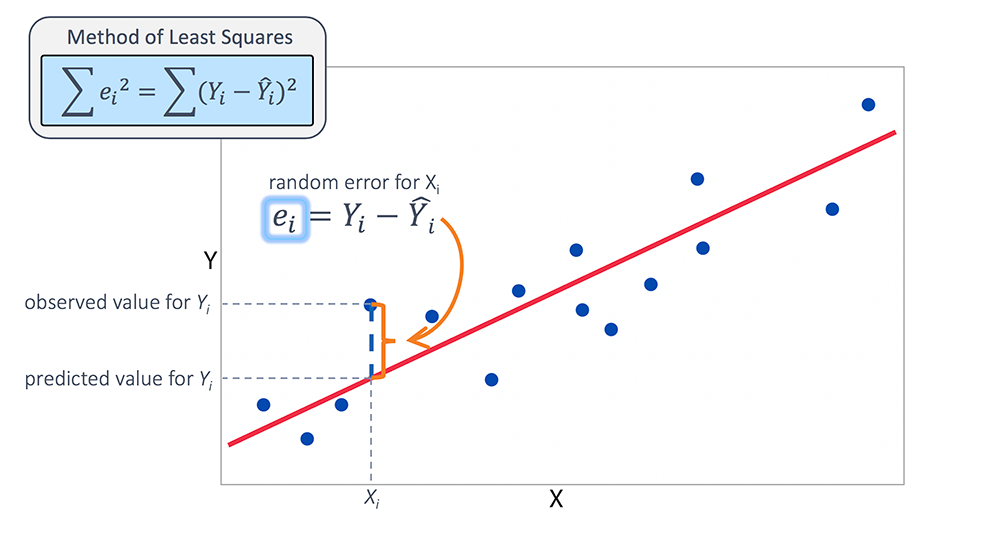
\includegraphics[width=7cm, height=4cm]{Figs/1.png}
			\caption{Simple Linear Regression, \href{https://tinyurl.com/2fvj5eh9}{Source}}
	\end{figure}

}

%%%%%%%%%%%%%%%%%%%%%%%%%%%%%%%%%%%%%%%%%%%%%%%%%%%%%%%%%%%%%%%%%%%%
\frame{\frametitle{Non-Geometric Approach}
	\begin{itemize} 
	
	\item \href{https://www.math.uwaterloo.ca/~hwolkowi/matrixcookbook.pdf}{Differentiating} this term and setting it to zero, we find that the estimate for $\beta$, which minimizes the squared error, satisfies the so-called \tc{keywords}{Normal} equation:
	\begin{equation*}
		X^T X \hat{\beta}=X^T Y
	\end{equation*}

	\item Provided $X^T X$ is invertible,
		\begin{equation*}
			\hat{\beta}=\left(X^T X\right)^{-1} X^T Y
		\end{equation*}

	\item We can then get the fitted values, $\hat{Y}$, and residuals, $\hat{\epsilon}$,
		\begin{equation*}
			\begin{gathered}
				\hat{Y}=X \hat{\beta}=X\left(X^T X\right)^{-1} X^T Y=H Y \\
				\hat{\epsilon}=Y-X \hat{\beta}=Y-\hat{Y}=(I-H) Y
			\end{gathered}
		\end{equation*}
	where the projection matrix $H=X\left(X^T X\right)^{-1} X^T$.

	\end{itemize}

}

%%%%%%%%%%%%%%%%%%%%%%%%%%%%%%%%%%%%%%%%%%%%%%%%%%%%%%%%%%%%%%%%%%%%
\frame{\frametitle{Geometric Approach}
	\begin{itemize} 
		\item Another way of looking at this problem is to say we want a solution (our fitted values) that lies in the space spanned by $X$ become as close as possible to $Y$.
		
		\item In this way, the systematic component $X \hat{\beta}$ is the projection of $Y$ onto the space spanned by $X$, and the residuals are $Y-X \hat{\beta}$. 
		
			\begin{figure}[H]
					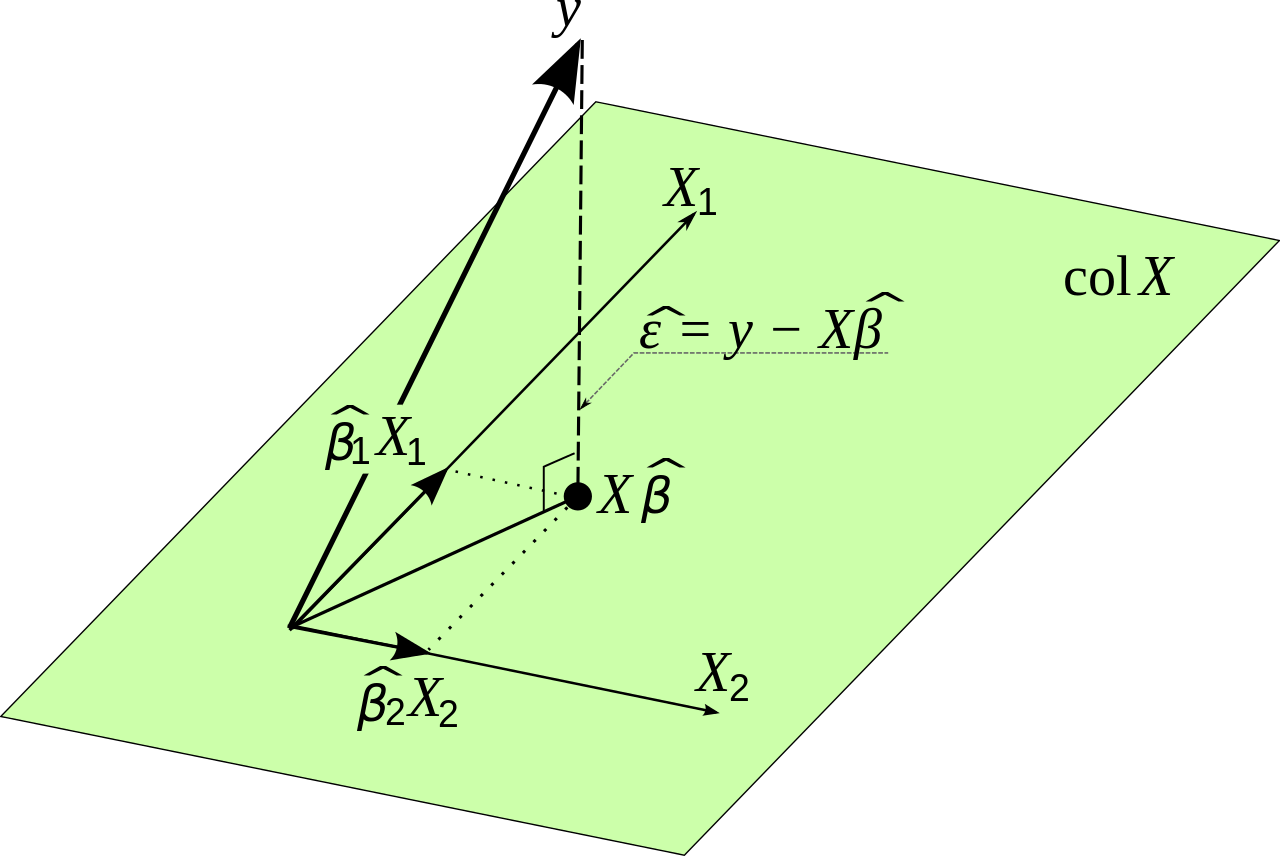
\includegraphics[width=6cm, height=4cm]{Figs/2.png}
					\caption{Geometric Approach of Linear Regression, \href{https://tinyurl.com/2zp8v79c}{Source}}
			\end{figure}
		
	\end{itemize}
}

%%%%%%%%%%%%%%%%%%%%%%%%%%%%%%%%%%%%%%%%%%%%%%%%%%%%%%%%%%%%%%%%%%%%

\frame{\frametitle{Extended Versions}
	\begin{itemize}
		
		\item The Ridge estimate of the linear regression problem is defined as:
		\begin{equation*}
			\begin{aligned}
				\hat{\beta}_{\text {Ridge }} &=\underset{\beta \in
					\mathbb{R}^n}{\operatorname{argmin}}\|y-X \beta\|_2^2+\frac{1}{2}\lambda \sum_{j=1}^n\left|\beta_j\right|^2 \\
				&=\underset{\beta \in \mathbb{R}^n}{\operatorname{argmin}} \| y-\left.X \beta\right|_2 ^2+\frac{1}{2}\lambda \|\beta\|_2^2
			\end{aligned}
		\end{equation*}

	\item The Lasso estimate of the linear regression problem is defined as:
		\begin{equation*}
			\begin{aligned}
				\hat{\beta}_{\text {Lasso }} &=\underset{\beta \in
					\mathbb{R}^n}{\operatorname{argmin}}\|y-X \beta\|_2^2+\lambda \sum_{j=1}^n\left|\beta_j\right| \\
				&=\underset{\beta \in \mathbb{R}^n}{\operatorname{argmin}} \| y-\left.X \beta\right|_2 ^2+\lambda \|\beta\|_1
			\end{aligned}
		\end{equation*}
	\end{itemize}

}
%%%%%%%%%%%%%%%%%%%%%%%%%%%%%%%%%%%%%%%%%%%%%%%%%%%%%%%%%%%%%%%%%%%%
\frametitle{Final Notes}
\centering
\vspace{50 pt}
\textbf{Thank You!}
\vspace{50pt}

\textbf{Any Question?}
%%%%%%%%%%%%%%%%%%%%%%%%%%%%%%%%%%%%%%%%%%
\end{document}